% !TEX root = ../main.tex
\clearpage
\appendix
\section{Training Curves}
We provide training loss curves of SimCLR, GIM and \ours{} for a better understanding of the
performance gap between them. Contrastive losses computed using outputs from the full ResNet-50
encoder are shown in Fig.~\ref{fig:loss_curve}. For GIM and \ours{}, losses from other decoders,
including {\em res2}, {\em res3}, {\em res4}, are also provided. As we can see in
Fig.~\ref{fig:loss_curve}, the losses of different decoders in \ours{}  closely match the loss of
the decoder in SimCLR during training, with the exception of {\em res2}, while for GIM this is not
the case.

\iflatexml
    \begin{figure}
    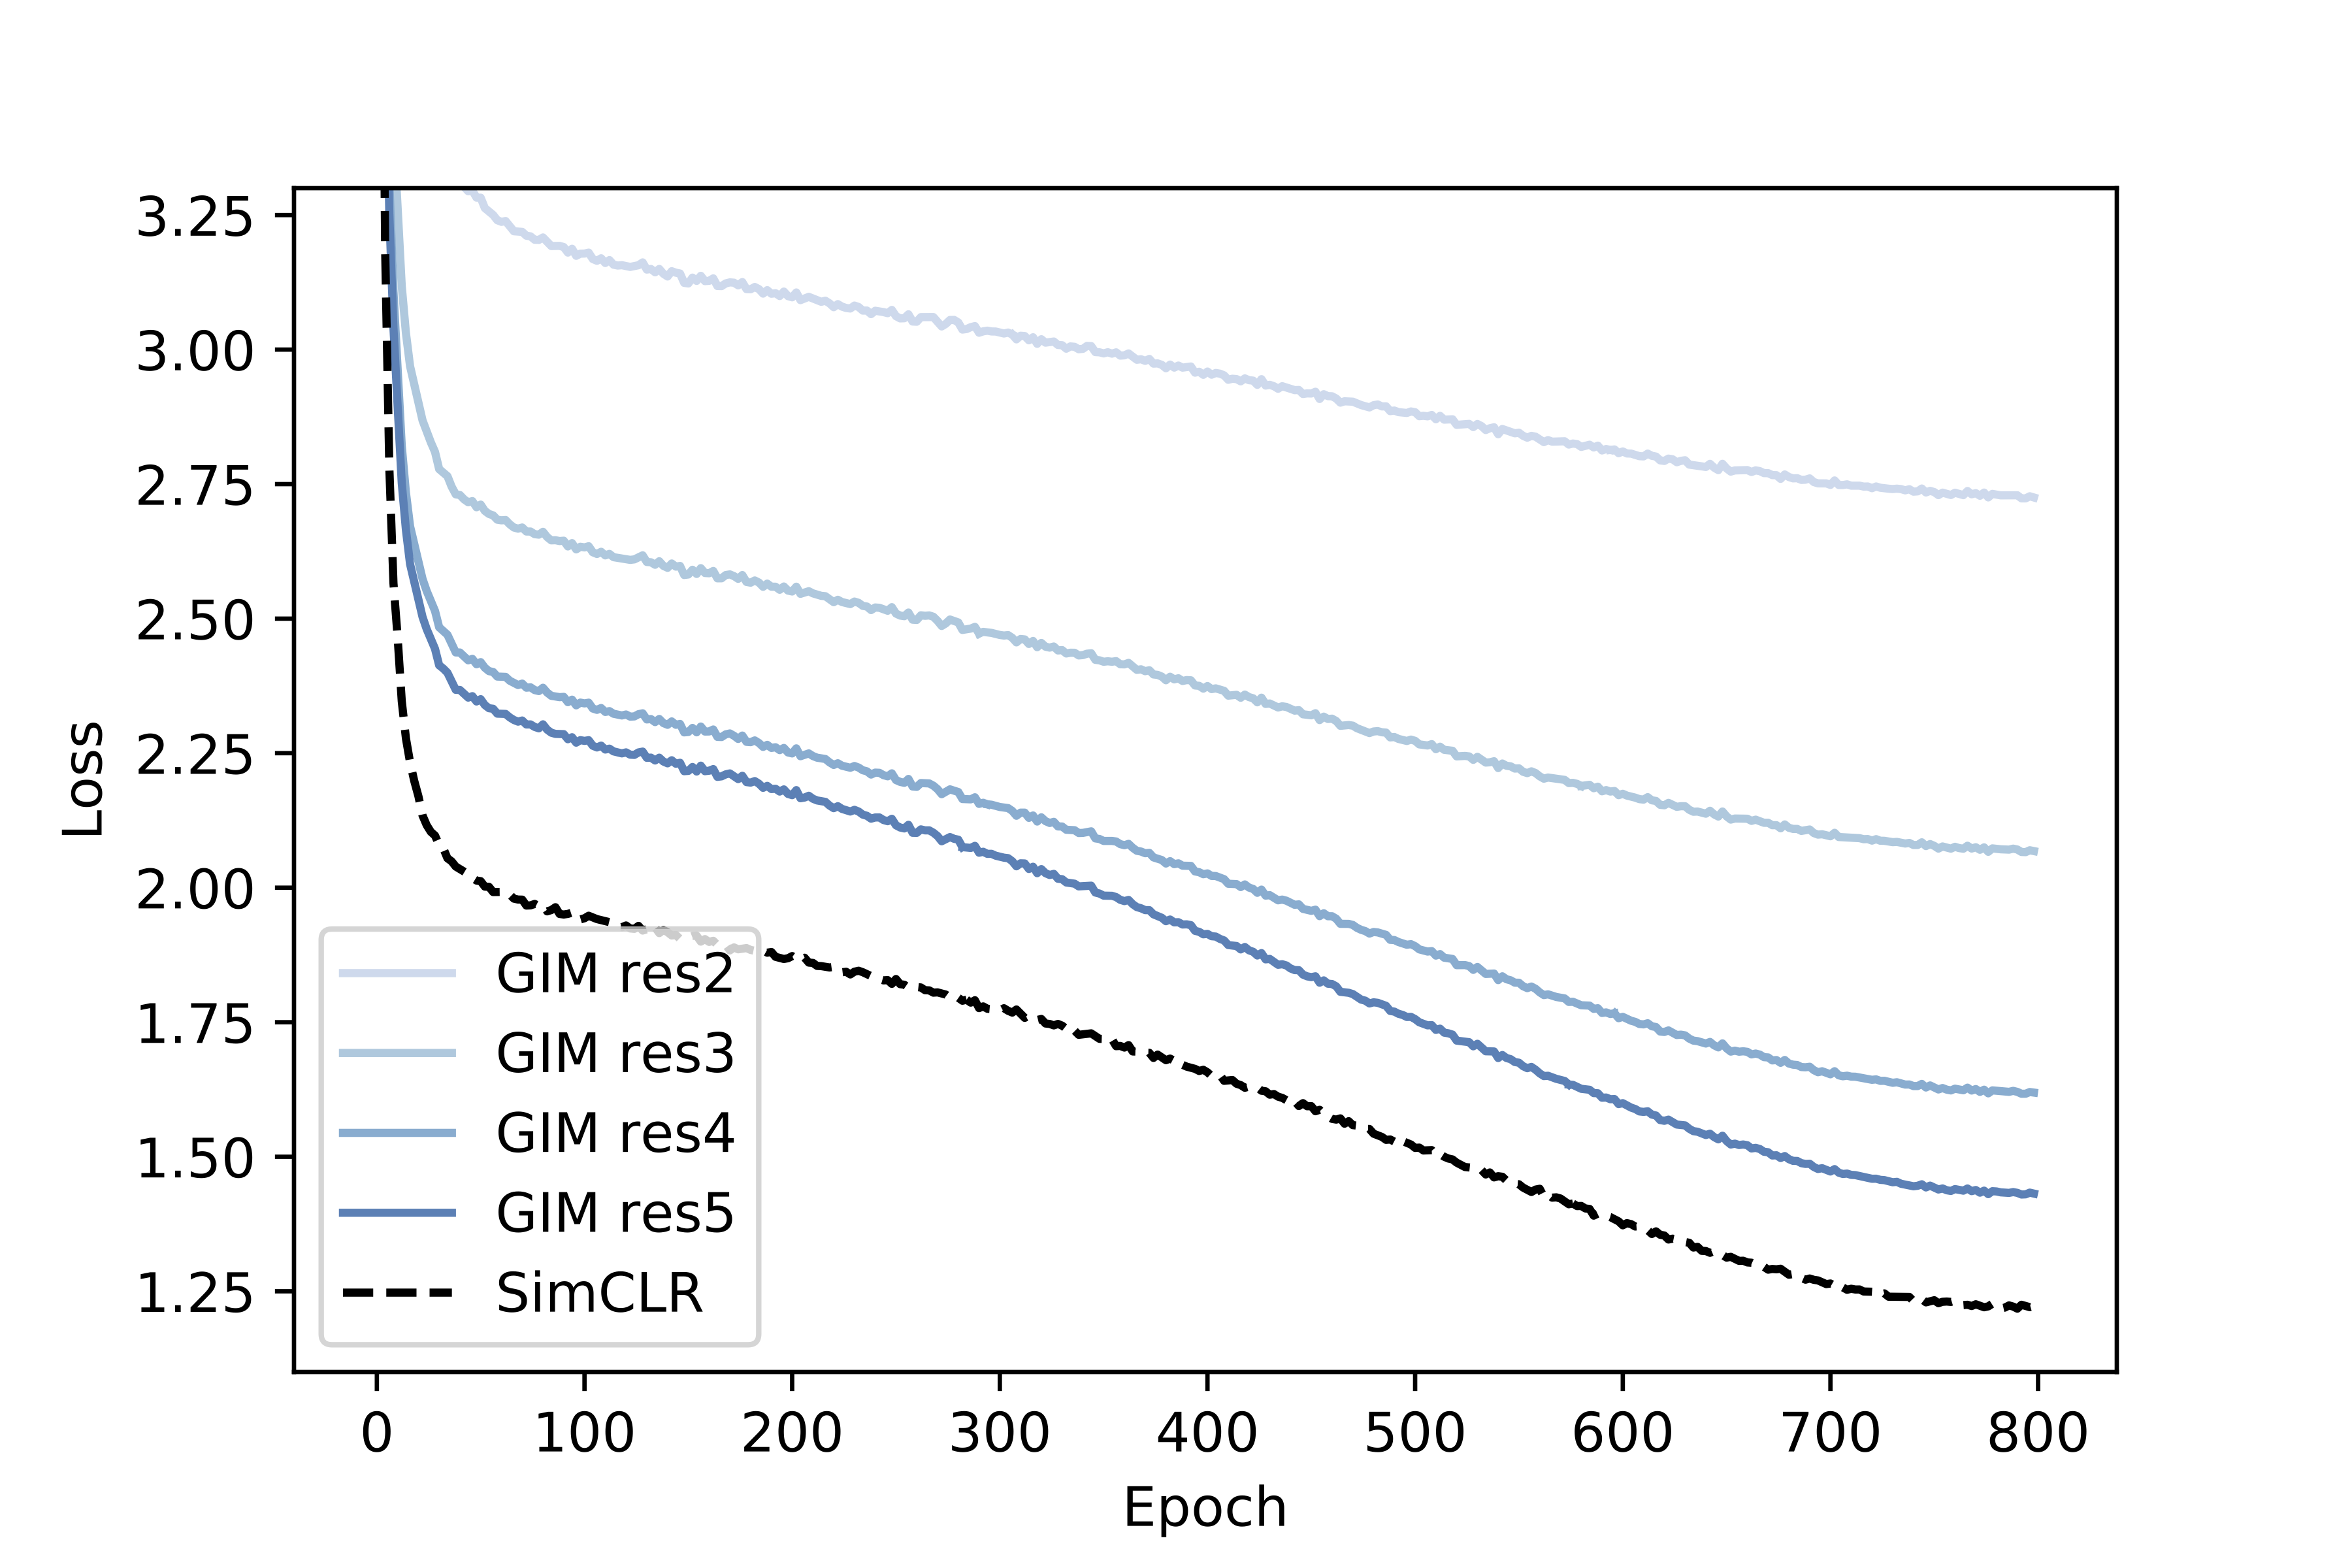
\includegraphics[width=3\linewidth, trim={0.3cm 0 1cm 0}, clip]{figures/simclr_vs_gim.png}
    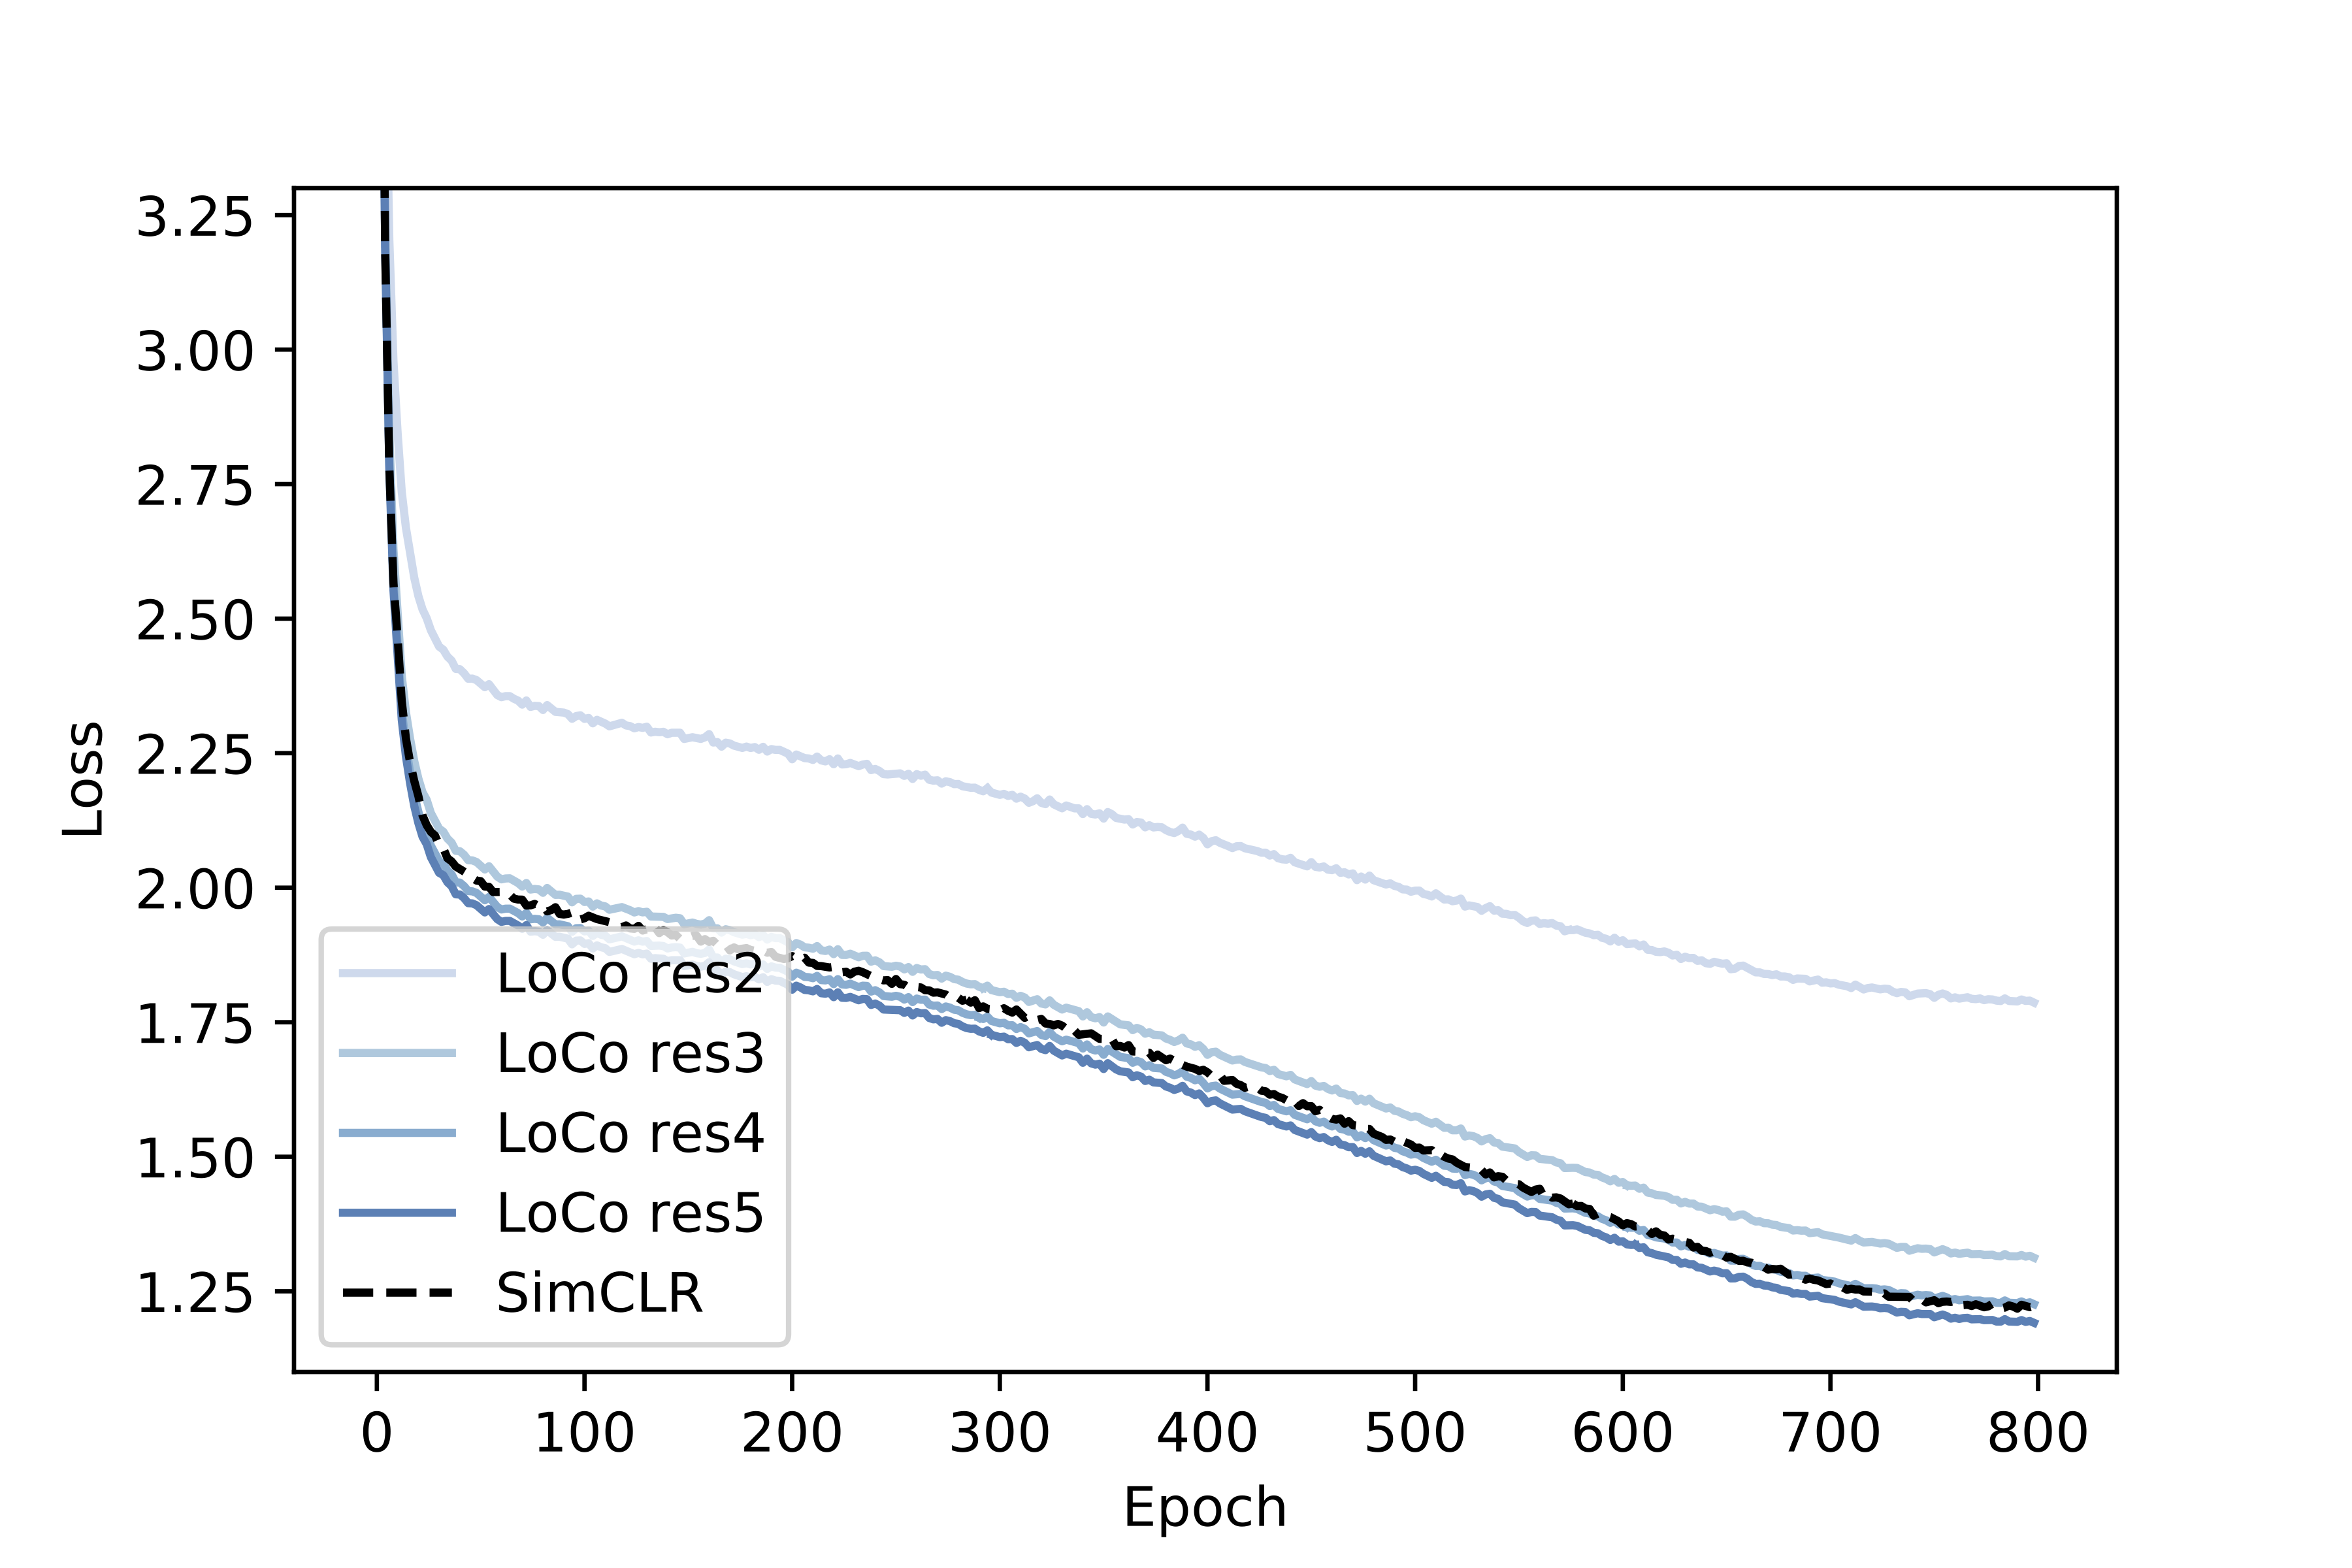
\includegraphics[width=3\linewidth, trim={0.3cm 0 1cm 0}, clip]{figures/simclr_vs_ours.png}
    \caption{Training loss curves for SimCLR, GIM and \ours{}}
    \label{fig:loss_curve}
    \end{figure}
\else
    \begin{figure}[htbp]
    \centering
    \begin{minipage}[t]{0.48\linewidth}
    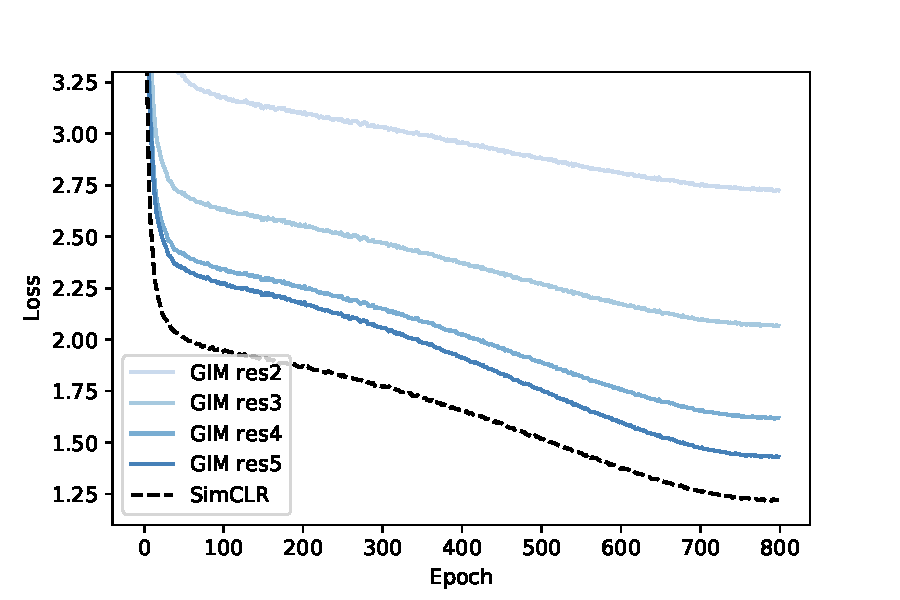
\includegraphics[width=1\linewidth, trim={0.3cm 0 1cm 0}, clip]{figures/simclr_vs_gim.pdf}
    \end{minipage}
    \hfill
    \begin{minipage}[t]{0.48\linewidth}
    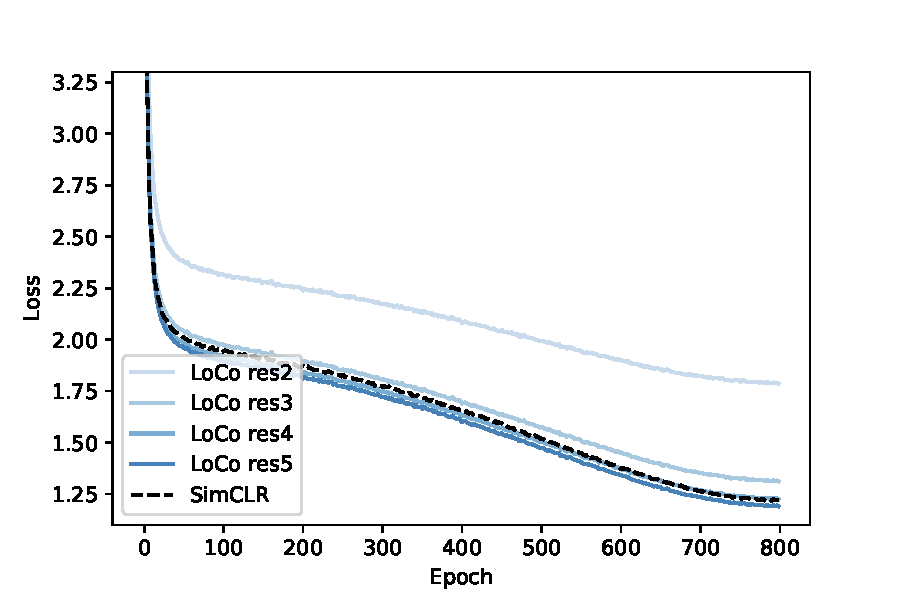
\includegraphics[width=1\linewidth, trim={0.3cm 0 1cm 0}, clip]{figures/simclr_vs_ours.pdf}	
    \end{minipage}
    \caption{Training loss curves for SimCLR, GIM and \ours{}}
    \label{fig:loss_curve}
    \end{figure}
\fi


\section{Architecture of Progressive ResNet-50}

In this section we show the block structure of each stage in Progressive ResNet-50 in
Table~\ref{tab:presnet_arch}. The block structure of ResNet-50 is also shown here for reference. We
downsample the feature map size progressively using bilinear interpolation, and  use basic blocks to
reduce the memory footprint of earlier stages, and group convolution to reduce the computation cost
of later stages to get a model with more balanced computation and memory footprint at each stage. We
use this model to show the great potential of \ours{} in terms of both memory saving and computation
for model parallelism. As it is designed to have 15\textasciitilde 20 memory footprint and
computation cost per stage, the peak memory usage will be significantly reduced in local learning,
and no worker that handles a stage of the encoder will become a computation bottleneck in model
parallelism.

\begin{table}[htbp]

\centering
\begin{tabular}{|c|c|c|c|c|}
\hline
\multirow{2}*{layer}     &  \multicolumn{2}{c|}{PResNet-50} & \multicolumn{2}{c|}{ResNet-50} \\ 
\cline{2-5} & output size & block structure & output size & block structure\\
\hline
conv1  & 112$\times$112    & 7x7, 32, stride 2 & 112$\times$112 &  7$\times$7, 64, stride 2  \\ 
\hline
\multirow{2}{*}{res2\_x} & \multirow{2}{*}{56$\times$56} & 3$\times$3 max pool, stride 2 & \multirow{2}{*}{56$\times$56} & 3$\times$3 max pool, stride 2\\ 
\cline{3-3} \cline{5-5} &                        
& \begin{math} \left[ \begin{tabular}[c]{@{}c@{}}3$\times$3, 56\\ 3$\times$3, 56\end{tabular}  \right ] \end{math}$\times$3  & ~ & \begin{math} \left[ \begin{tabular}[c]{@{}c@{}}1$\times$1, 64\\ 3$\times$3, 64\\ 1$\times$1, 256 \end{tabular}  \right ] \end{math}$\times$3   \\ 
\hline
res3\_x                  
& 36$\times$36 
& \begin{math} \left[ \begin{tabular}[c]{@{}c@{}}3$\times$3, 96\\ 3$\times$3, 96 \end{tabular} \right ] \end{math}$\times$3 
& 28$\times$28 
&  \begin{math} \left[  \begin{tabular}[c]{@{}c@{}}1$\times$1, 128\\  3$\times$3, 128\\ 1$\times$1, 512 \end{tabular}  \right ] \end{math}$\times$4  \\ 
\hline
res4\_x                  & 24$\times$24                  
& \begin{math} \left[ \begin{tabular}[c]{@{}c@{}}1$\times$1, 144\\ 3$\times$3, 144\\ 1$\times$1, 576 \end{tabular} \right ] \end{math}$\times$3 
& 14$\times$14
& \begin{math} \left[ \begin{tabular}[c]{@{}c@{}}1$\times$1, 256\\  3$\times$3, 256\\ 1$\times$1, 1024 \end{tabular} \right ] \end{math}$\times$6 \\ 
\hline
res5\_x                  & 16$\times$16                    
& \begin{tabular}[c]{@{}c@{}} \begin{math} \left[ \begin{tabular}[c]{@{}c@{}}1$\times$1, 256, 2 grps\\ 3$\times$3, 256, 2 grps\\ 1$\times$1, 1024 \end{tabular} \right ] \end{math}$\times$1 \\ \begin{math} \left[ \begin{tabular}[c]{@{}c@{}}1$\times$1, 256, 2 grps\\ 3$\times$3, 256, 2 grps\\ 1$\times$1, 1024, 2 grps \end{tabular} \right ] \end{math}$\times$2\end{tabular}
& 7$\times$7
& \begin{math} \left[ \begin{tabular}[c]{@{}c@{}}1$\times$1, 512\\ 3$\times$3, 512\\ 1$\times$1, 2048 \end{tabular} \right ] \end{math}$\times$3 \\ \hline
res6\_x                  & 12$\times$12                    
& \begin{tabular}[c]{@{}c@{}} \begin{math} \left[ \begin{tabular}[c]{@{}c@{}}1$\times$1, 512, 16 grps\\ 3$\times$3, 512, 16 grps\\ 1$\times$1, 2048 \end{tabular} \right ] \end{math}$\times$1\\ \begin{math} \left[ \begin{tabular}[c]{@{}c@{}}1$\times$1, 512, 16 grps\\ 3$\times$3, 512, 16 grps\\ 1$\times$1, 2048, 16 grps \end{tabular} \right ] \end{math}$\times$2 \end{tabular} & - & -\\ \hline
res7\_x                  & 8$\times$8                    
& \begin{tabular}[c]{@{}c@{}} \begin{math} \left[ \begin{tabular}[c]{@{}c@{}}1$\times$1, 1024, 128 grps\\ 3$\times$3, 1024, 128 grps\\ 1$\times$1, 4096 \end{tabular} \right ] \end{math} $\times$1 \\ \begin{math} \left[ \begin{tabular}[c]{@{}c@{}}1$\times$1, 1024, 128 grps\\ 3$\times$3, 1024, 128 grps\\ 1$\times$1, 4096, 128 grps \end{tabular} \right ] \end{math} $\times$2 \end{tabular} & -  & -\\ 
\hline
                          & 1$\times$1                    & average pool, 1000-d fc & 1$\times$1 & average pool, 1000-d fc                                                                                                                                                                                                                                                                       \\ \hline
\end{tabular}
\vspace{0.1in}
\caption{Architectural details of Progressive ResNet-50 and ResNet-50. Output sizes for both models are specified individually}
\label{tab:presnet_arch}
\end{table}

\section{Representation visualization}

In this section we show some visualization results of the learned representation
of SimCLR, GIM and
\ours{}. We subsample images belonging to the first 10 classes of ImageNet-1K from
the validation set (500 images in total) and use t-SNE~\cite{maaten2008visualizing} to visualize the
4096-d vector representation from the PResNet-50 encoder. The results are shown in
Fig~\ref{fig:tsne_vis}. We can see \ours{} learns image
embedding vectors that can form more compact clusters compared to GIM.

\iflatexml
    \begin{figure}
    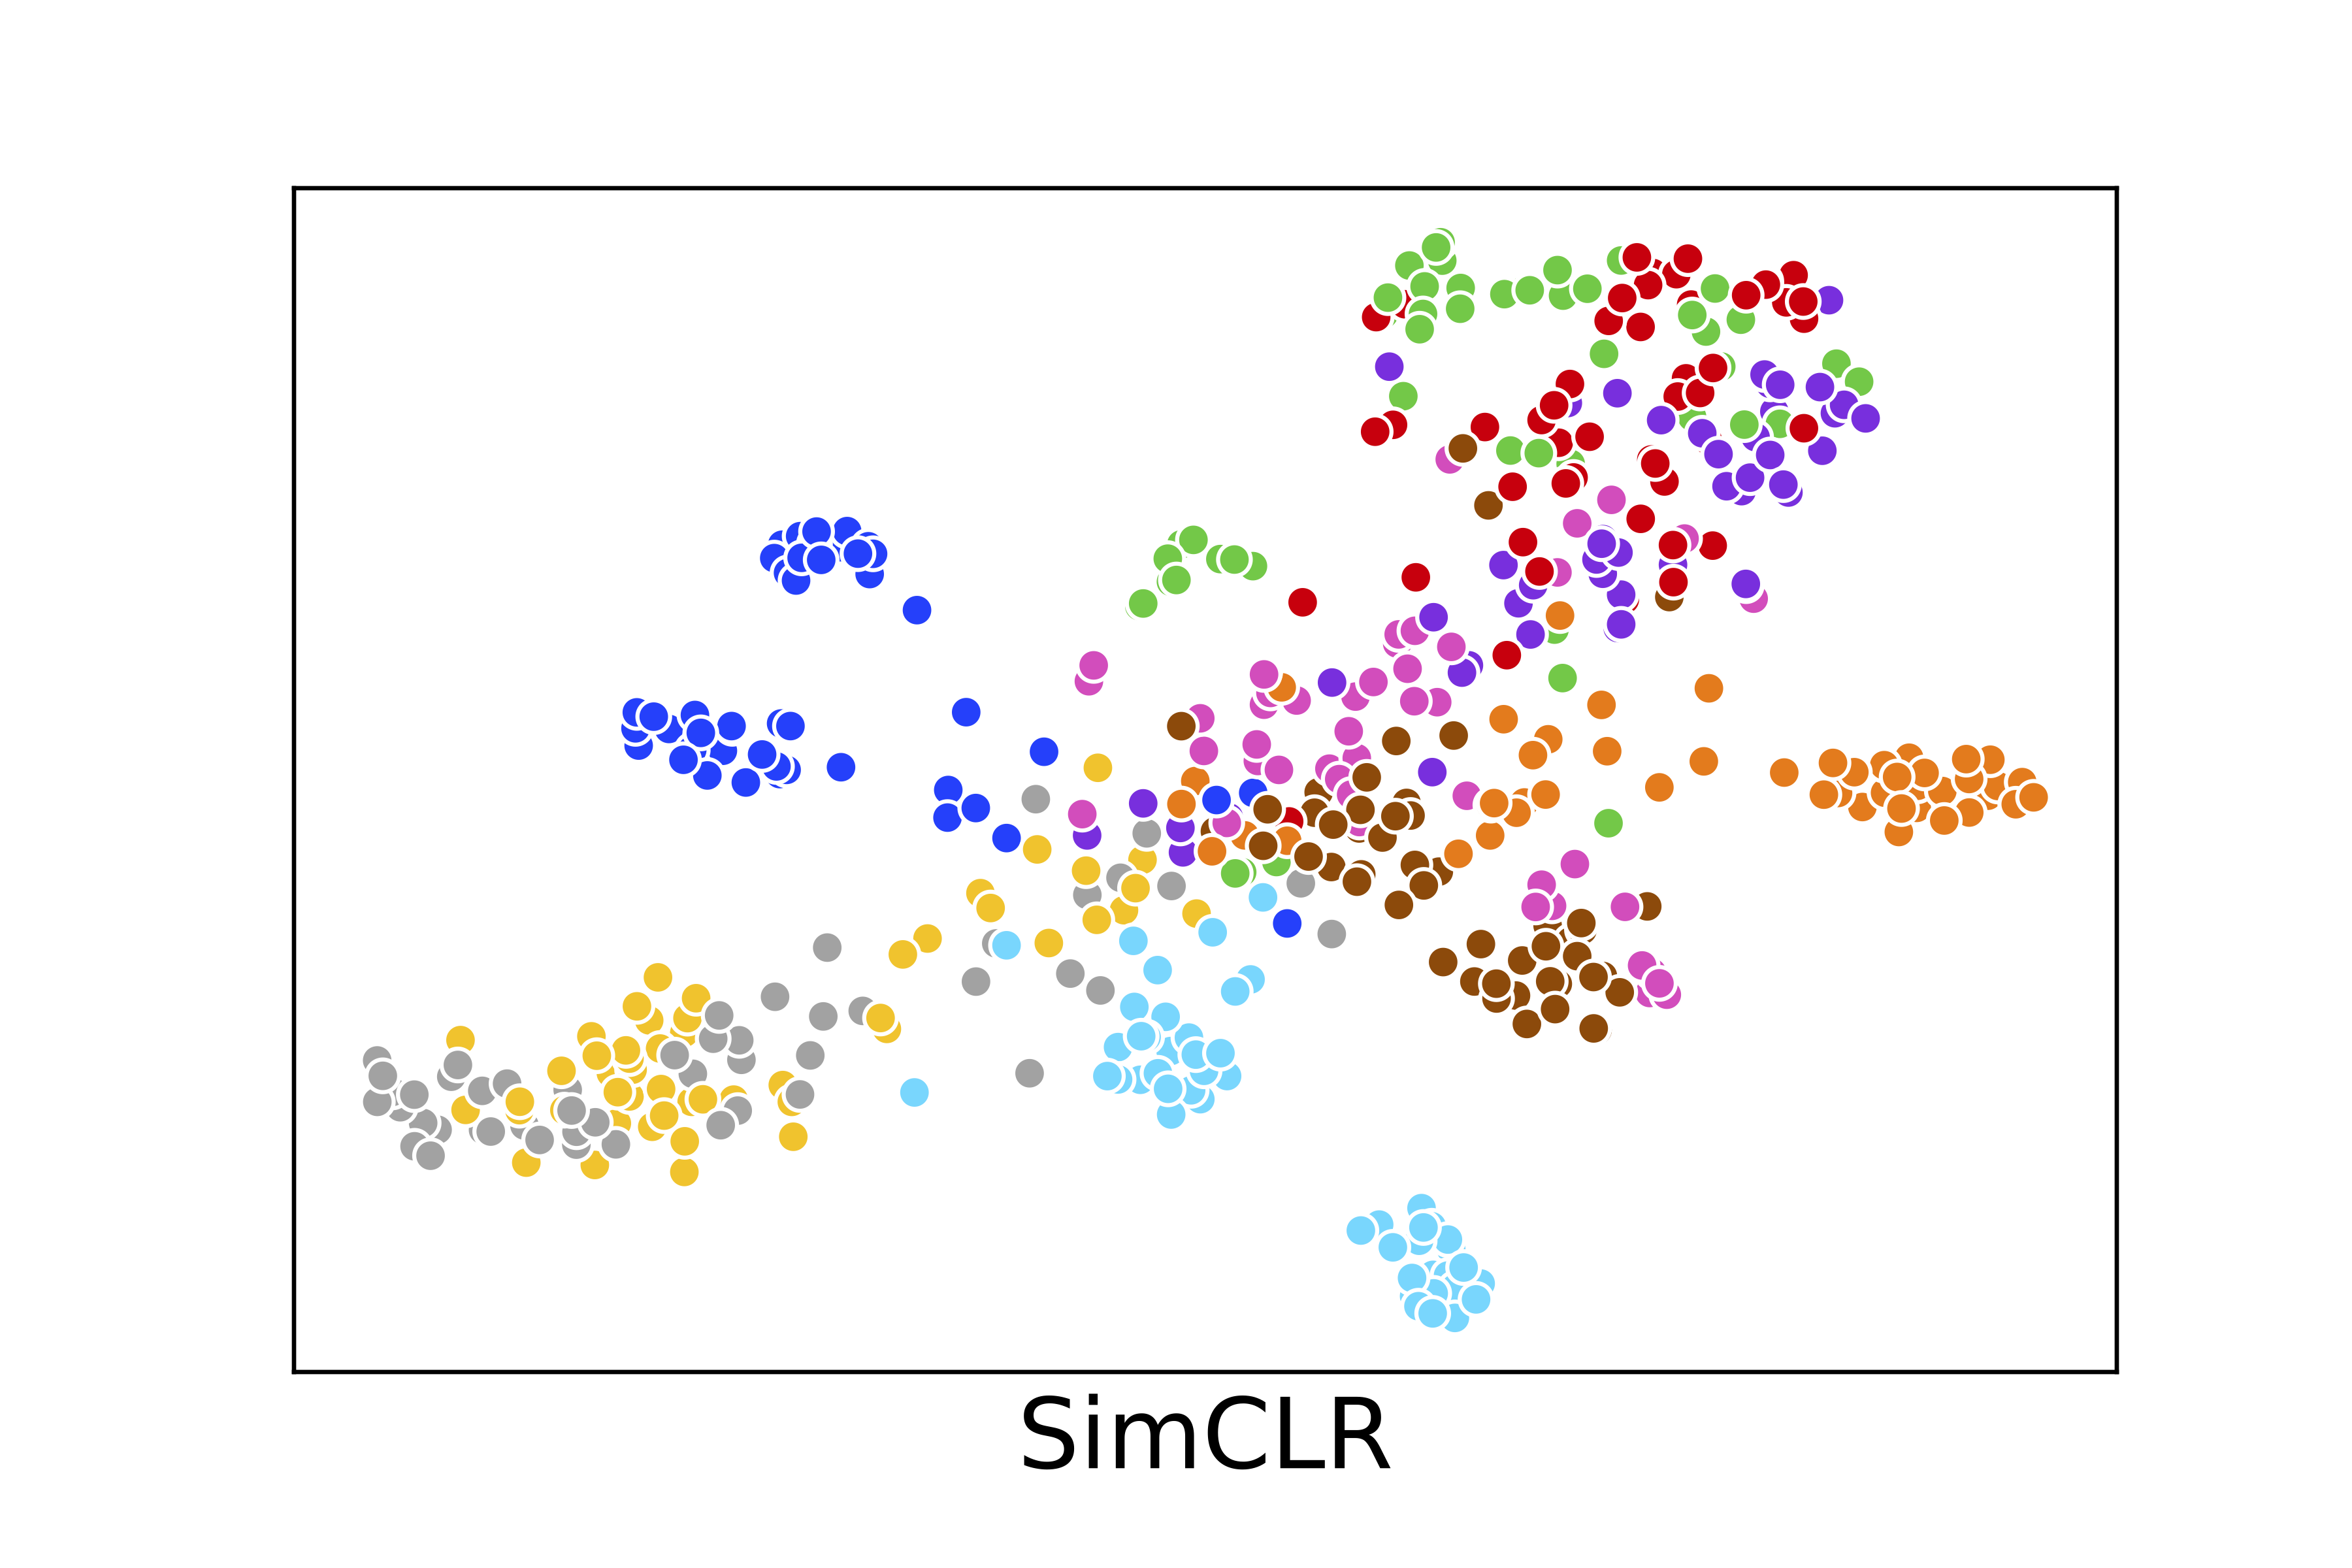
\includegraphics[width=2\linewidth, trim={1.9cm 0 1.5cm 0}, clip]{figures/simclr_tsne.png}
    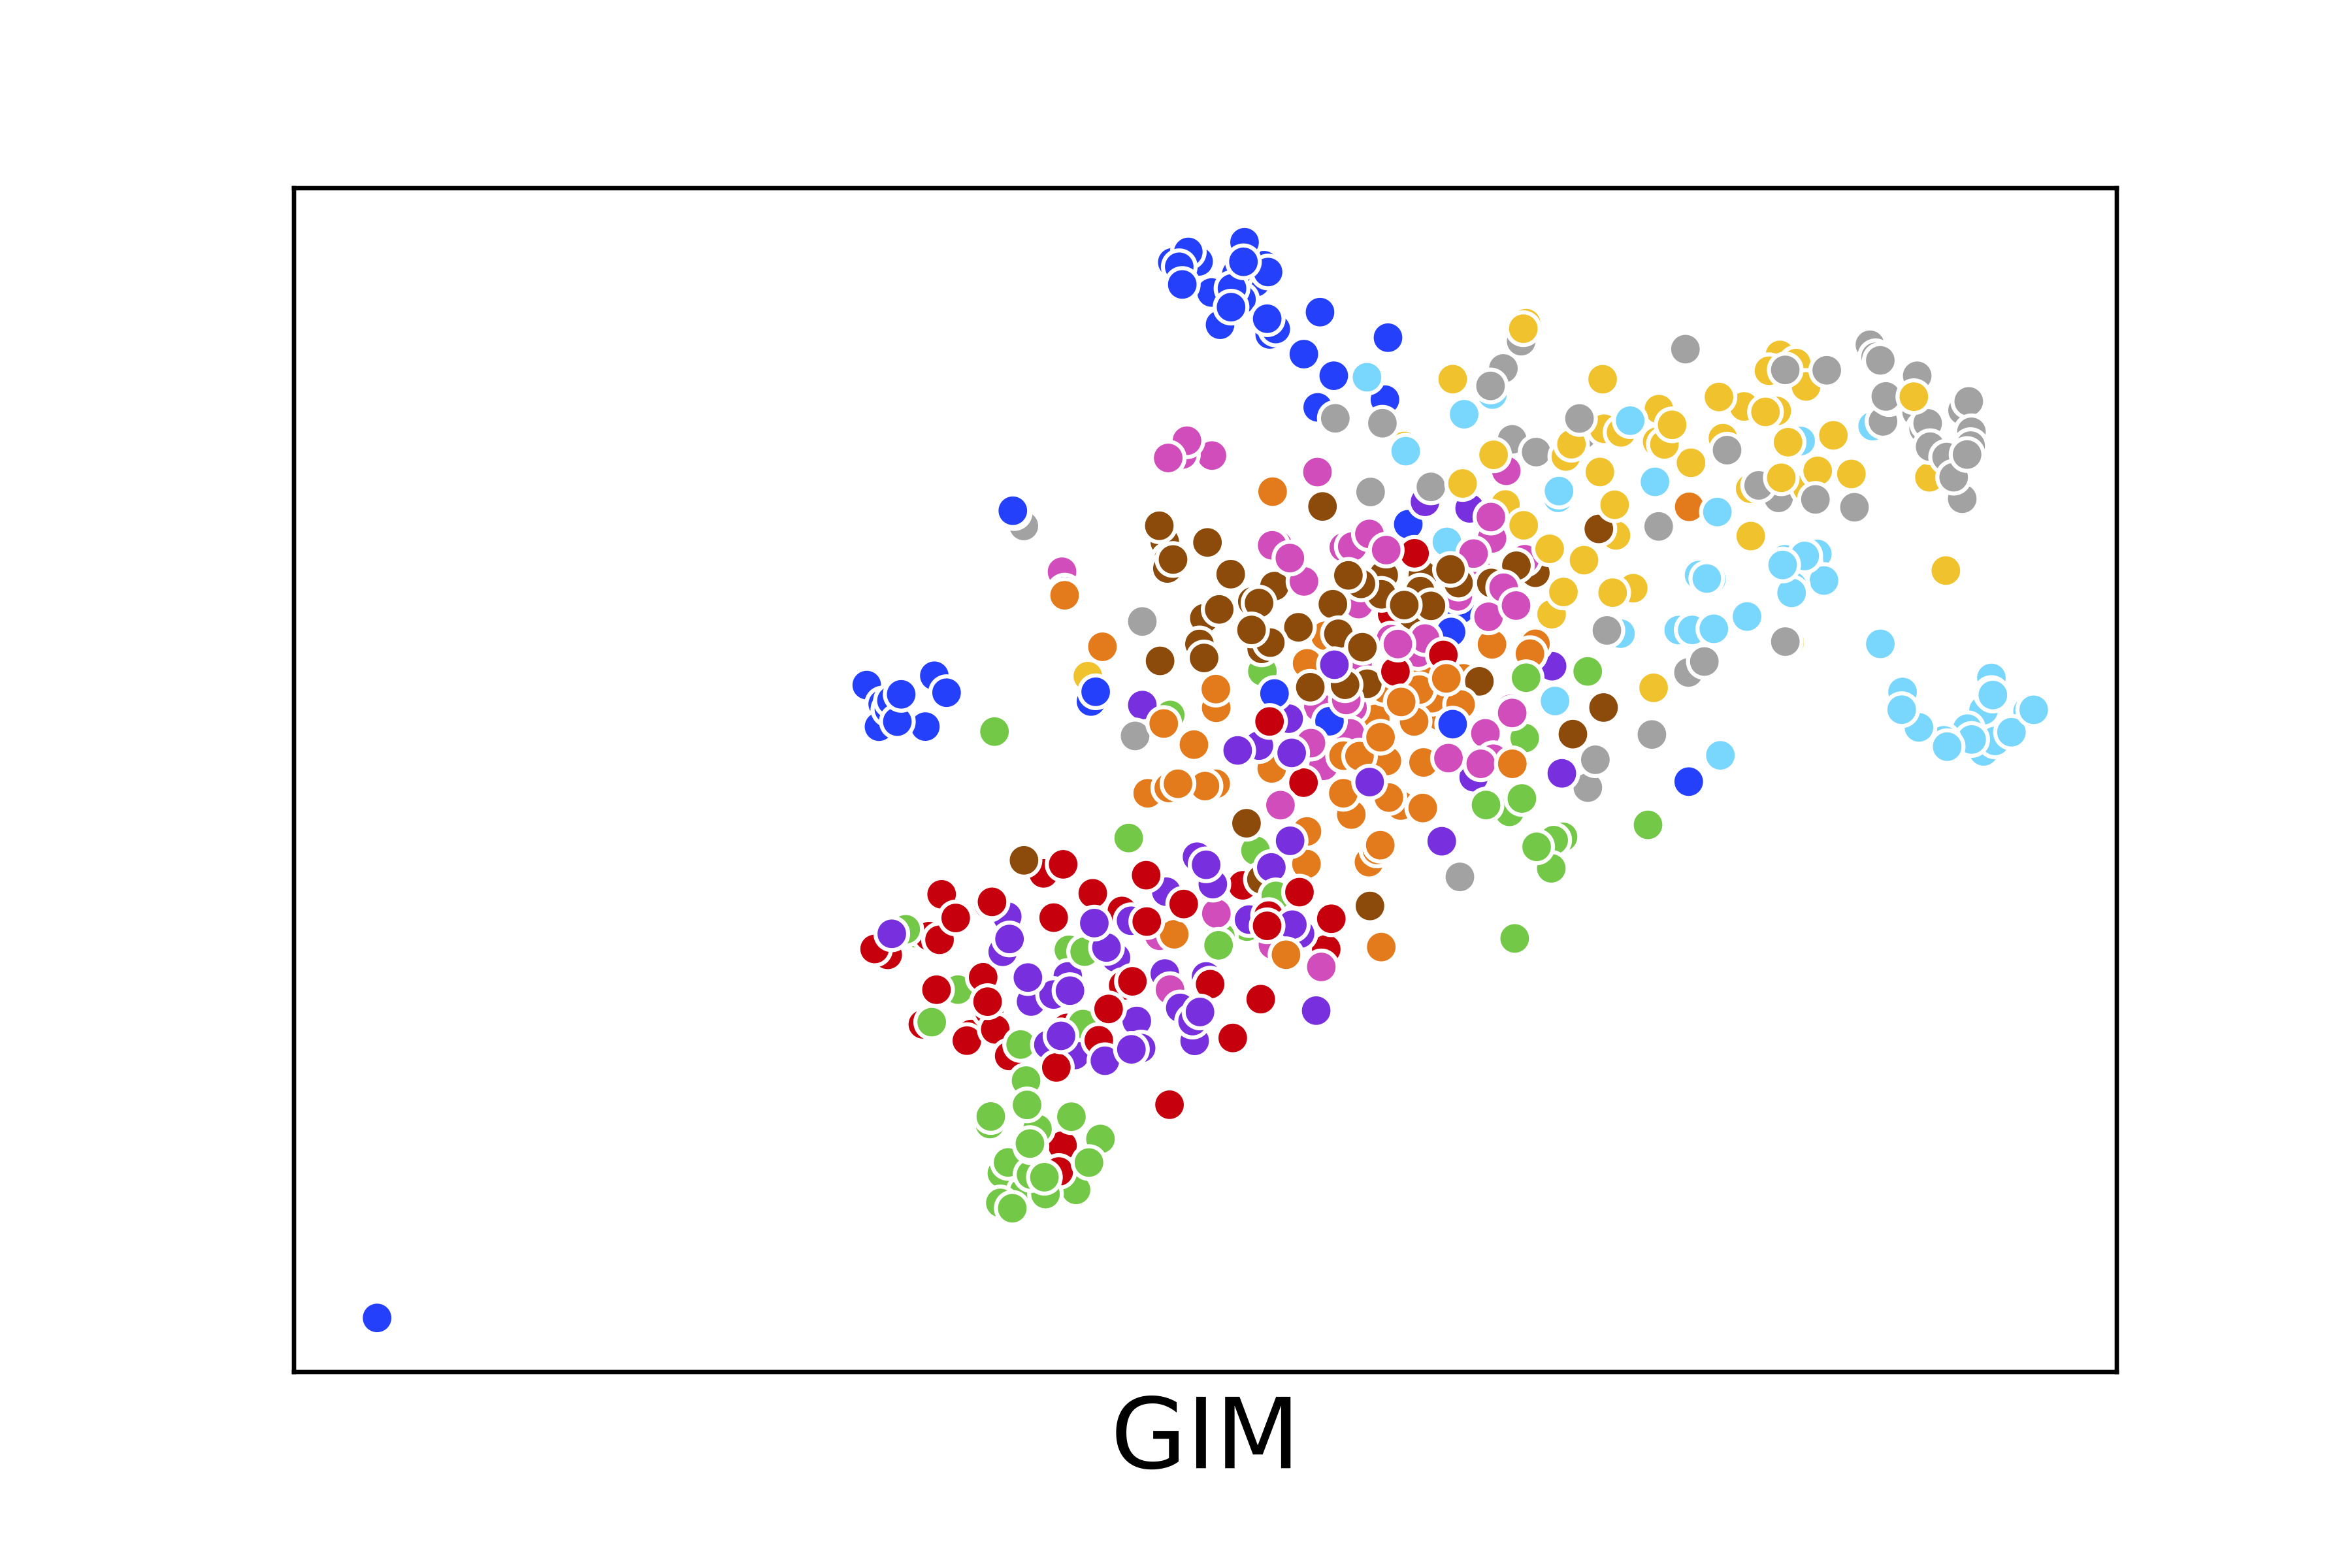
\includegraphics[width=2\linewidth, trim={1.9cm 0 1.5cm 0}, clip]{figures/gim_tsne.png}
    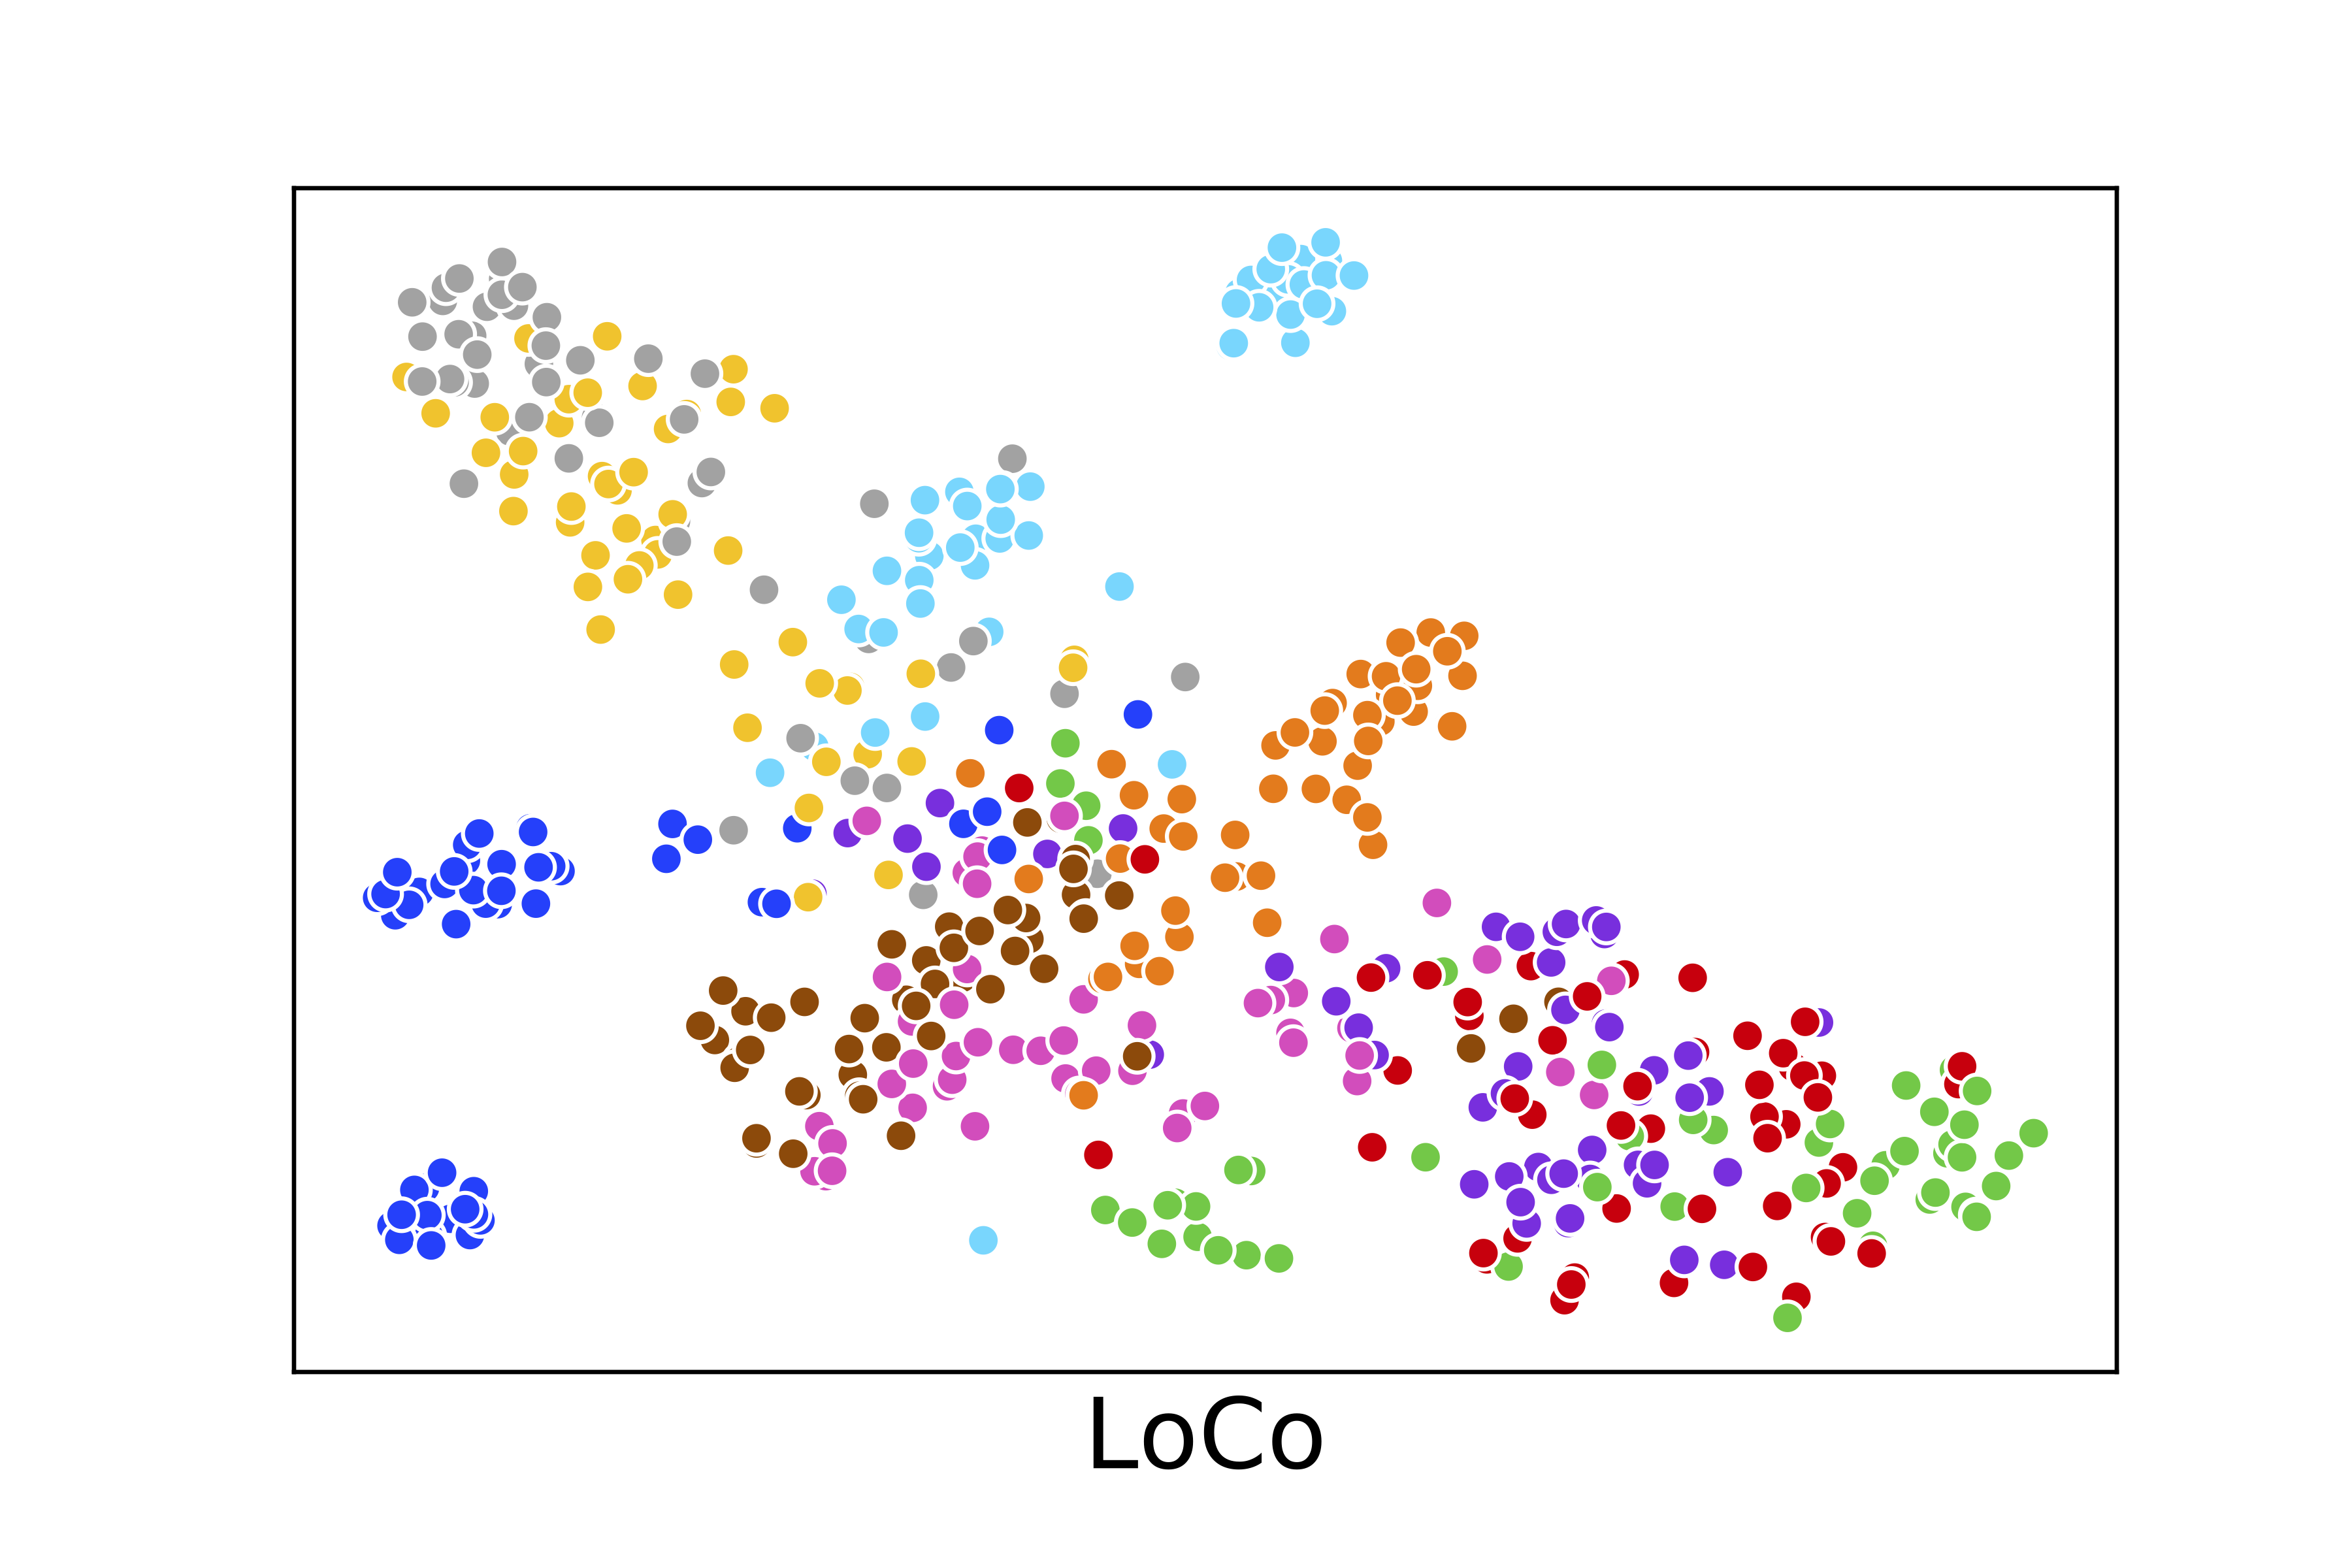
\includegraphics[width=2\linewidth, trim={1.9cm 0 1.5cm 0}, clip]{figures/loco_tsne.png}
    \caption{t-SNE visualization results for SimCLR, GIM and \ours{}}
    \label{fig:tsne_vis}
    \end{figure}
\else
    \begin{figure}[htbp]
    \centering
    \begin{minipage}[t]{0.31\linewidth}
    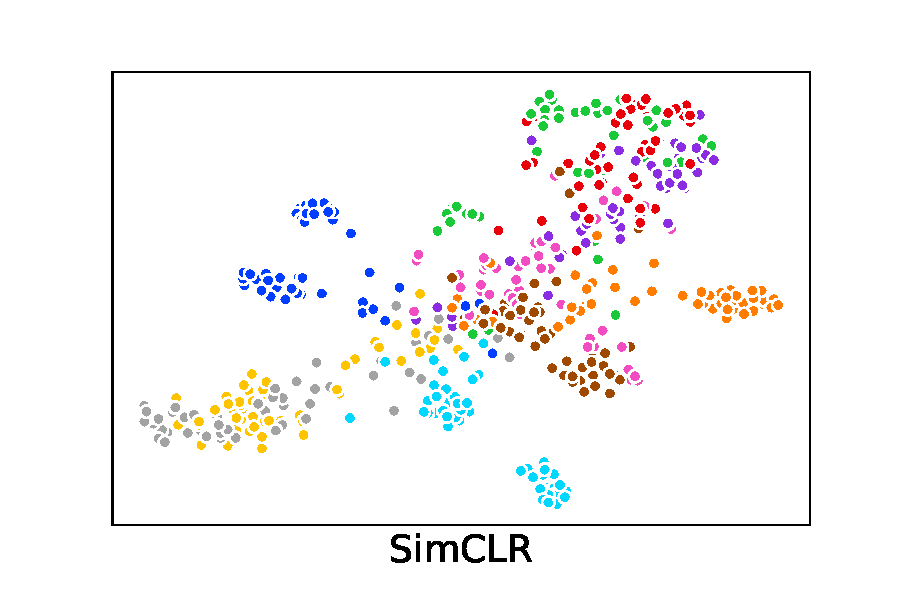
\includegraphics[width=1\linewidth, trim={1.9cm 0 1.5cm 0}, clip]{figures/simclr_tsne.pdf}
    \end{minipage}
    \hfill
    \begin{minipage}[t]{0.31\linewidth}
    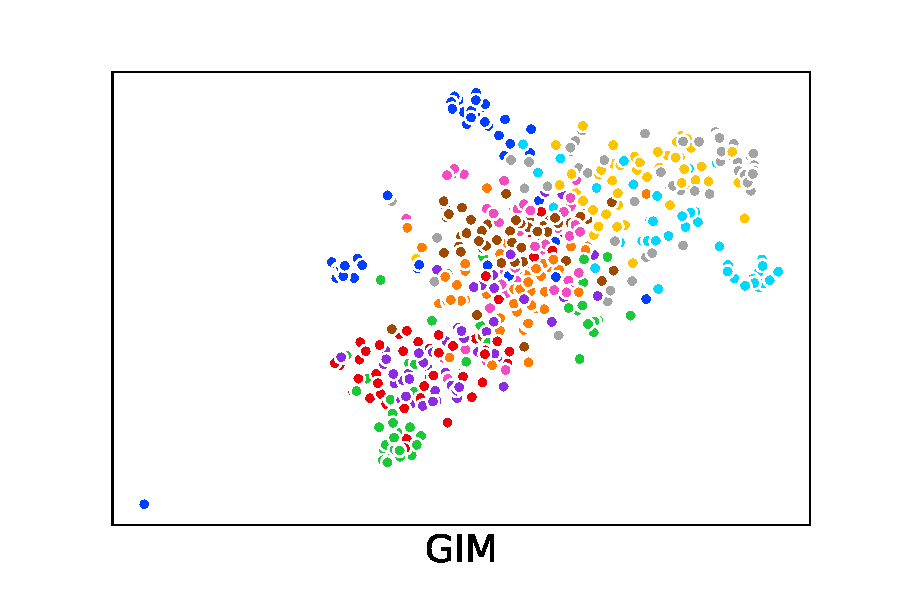
\includegraphics[width=1\linewidth, trim={1.9cm 0 1.5cm 0}, clip]{figures/gim_tsne.pdf}
    \end{minipage}
    \hfill
    \begin{minipage}[t]{0.31\linewidth}
    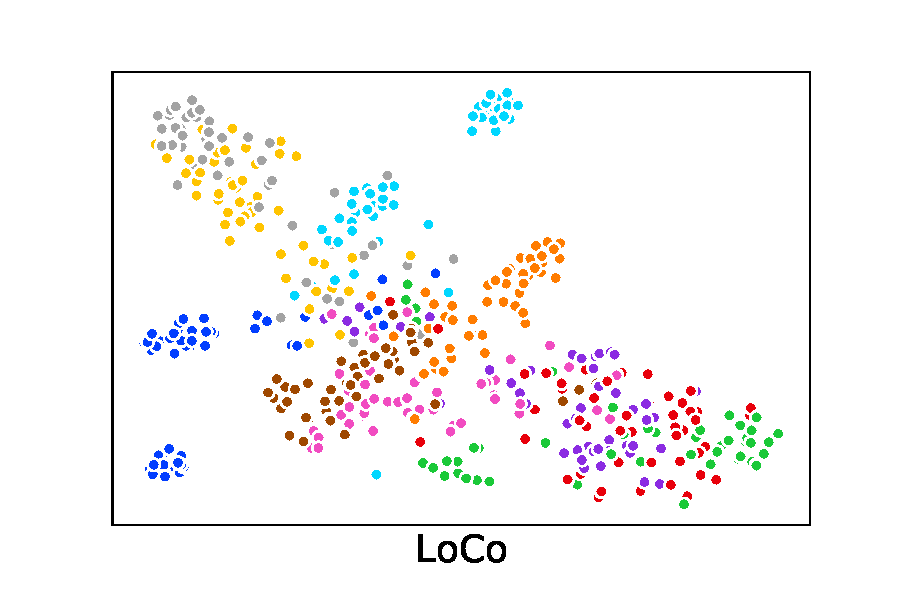
\includegraphics[width=1\linewidth, trim={1.9cm 0 1.5cm 0}, clip]{figures/loco_tsne.pdf}	
    \end{minipage}
    \caption{t-SNE visualization results for SimCLR, GIM and \ours{}}
    \label{fig:tsne_vis}
    \end{figure}
\fi

\clearpage

\section{Qualitative results for downstream tasks}

Last, we show qualitative results of detection and instance segmentation tasks on COCO in Fig.~\ref{fig:coco_vis}.

\begin{figure}[htbp]
\centering
\iflatexml
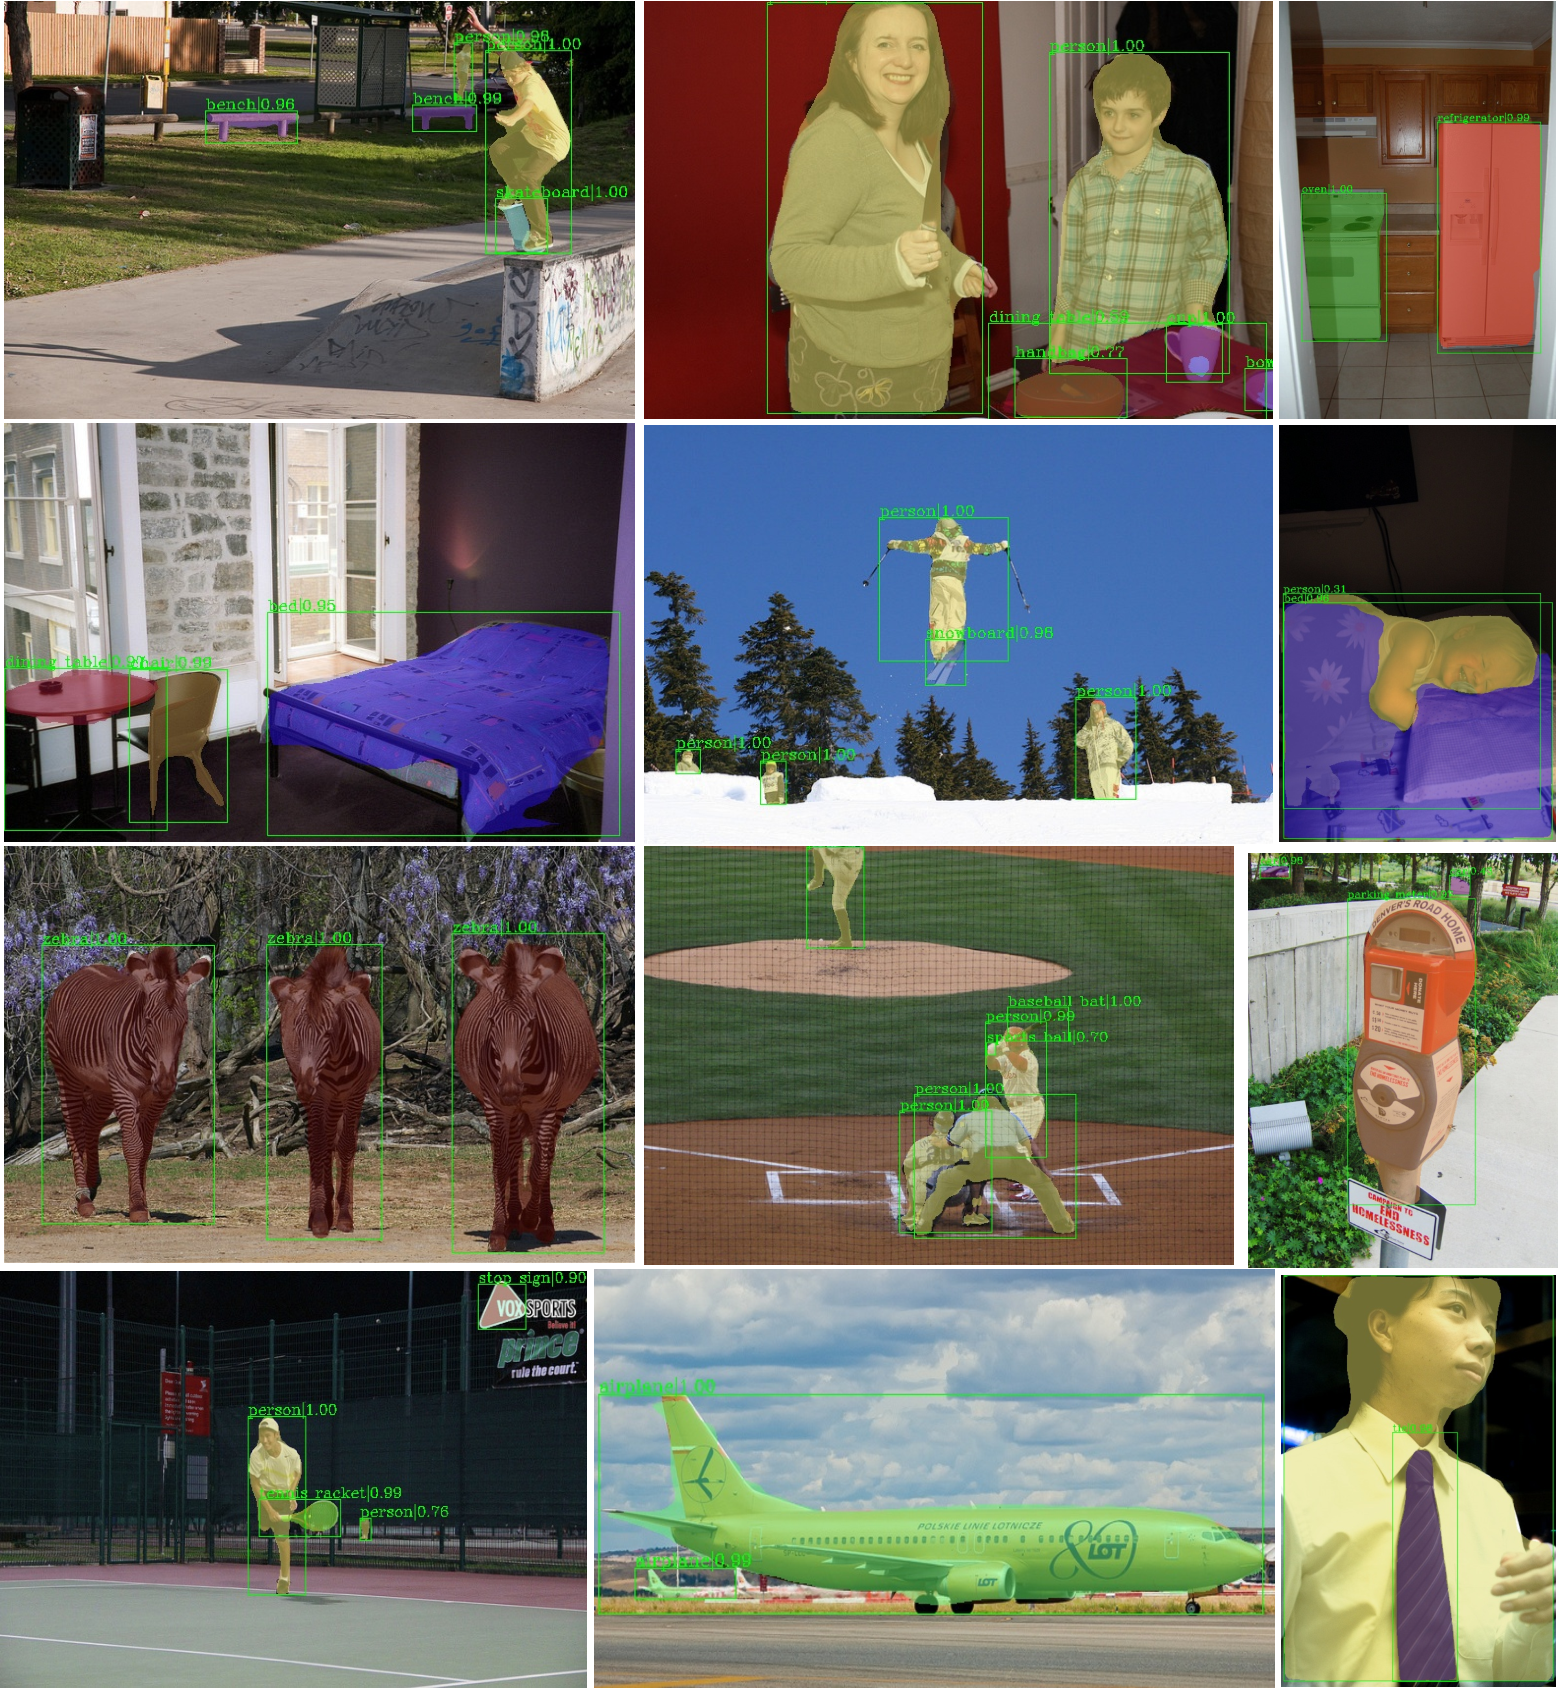
\includegraphics[width=6\linewidth]{figures/coco_vis.pdf}
\else
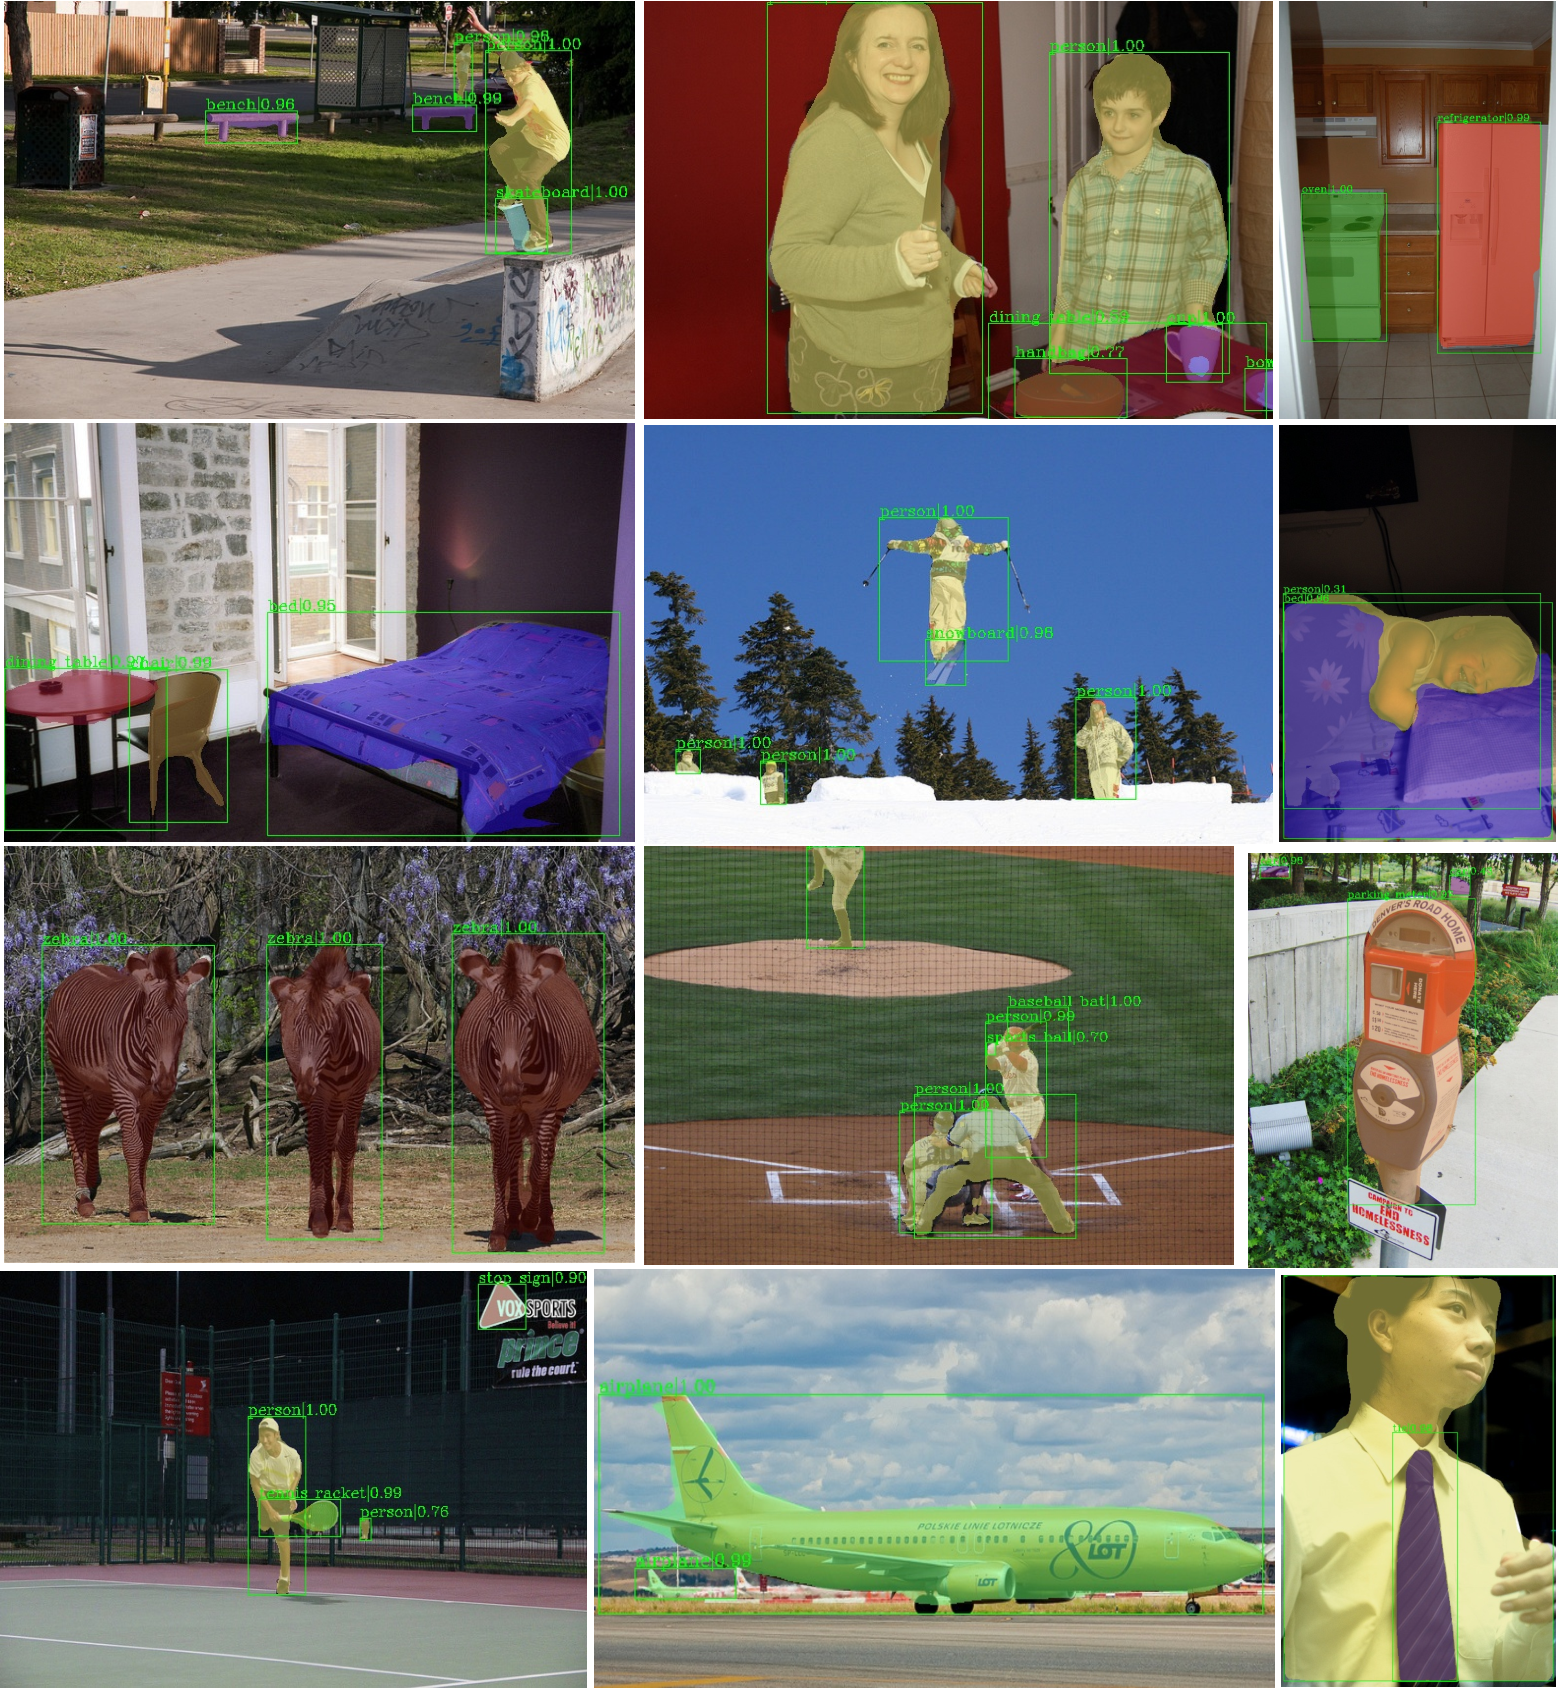
\includegraphics[width=1.0\linewidth]{figures/coco_vis.pdf}
\fi
\caption{Qualitative results on COCO-10K, \ours{} trained on 800 epochs with ResNet-50 is used to
initialize the Mask R-CNN model}
\label{fig:coco_vis}
\end{figure}


\newpage